\documentclass[12pt,a4paper]{article}
\usepackage{ctex}
\usepackage{algorithmic}
\usepackage{amsmath,amscd,amsbsy,amssymb,latexsym,url,bm,amsthm}
\usepackage{epsfig,graphicx,subfigure}
\usepackage{enumitem,balance}
\usepackage{wrapfig}
\usepackage{mathrsfs,euscript}
\usepackage[usenames]{xcolor}
\usepackage{hyperref}
\usepackage[vlined,ruled,linesnumbered]{algorithm2e}
\usepackage{array}
\hypersetup{colorlinks=true,linkcolor=black}

\newtheorem{theorem}{Theorem}
\newtheorem{lemma}[theorem]{Lemma}
\newtheorem{proposition}[theorem]{Proposition}
\newtheorem{corollary}[theorem]{Corollary}
\newtheorem{exercise}{Exercise}
\newtheorem*{solution}{Solution}
\newtheorem{definition}{Definition}
\theoremstyle{definition}

\renewcommand{\thefootnote}{\fnsymbol{footnote}}

\newcommand{\postscript}[2]
 {\setlength{\epsfxsize}{#2\hsize}
  \centerline{\epsfbox{#1}}}

\renewcommand{\baselinestretch}{1.0}

\setlength{\oddsidemargin}{-0.365in}
\setlength{\evensidemargin}{-0.365in}
\setlength{\topmargin}{-0.3in}
\setlength{\headheight}{0in}
\setlength{\headsep}{0in}
\setlength{\textheight}{10.1in}
\setlength{\textwidth}{7in}
\makeatletter \renewenvironment{proof}[1][Proof] {\par\pushQED{\qed}\normalfont\topsep6\p@\@plus6\p@\relax\trivlist\item[\hskip\labelsep\bfseries#1\@addpunct{.}]\ignorespaces}{\popQED\endtrivlist\@endpefalse} \makeatother
\makeatletter
\renewenvironment{solution}[1][Solution] {\par\pushQED{\qed}\normalfont\topsep6\p@\@plus6\p@\relax\trivlist\item[\hskip\labelsep\bfseries#1\@addpunct{.}]\ignorespaces}{\popQED\endtrivlist\@endpefalse} \makeatother

\begin{document}
\noindent

%========================================================================
\noindent\framebox[\linewidth]{\shortstack[c]{
\Large{\textbf{Lab11-NP Reduction}}\vspace{1mm}\\
CS214-Algorithm and Complexity, Xiaofeng Gao, Spring 2020.}}
\begin{center}
\footnotesize{\color{red}$*$ If there is any problem, please contact TA Shuodian Yu. }

\footnotesize{\color{blue}$*$ Name:Hongjie Fang  \quad Student ID:518030910150 \quad Email: galaxies@sjtu.edu.cn}
\end{center}
\begin{enumerate}
	\item What is the ``certificate'' and ``certifier'' for the following problems?
	\begin{enumerate}
		\item \emph{ZERO-ONE INTEGER PROGRAMMING}: Given an integer $m \times n$ matrix $A$ and an integer $m$-vector $b$, is there an integer $n$-vector $x$ with elements in the set $\{0, 1\}$ such that $Ax \leq b$.
		\item \emph{SET PACKING}: Given a finite set $U$, a positive integer $k$ and several subsets $U_1, U_2, \ldots, U_m$ of $U$, is there $k$ or more subsets which are disjoint with each other?
		\item \emph{STEINER TREE IN GRAPHS}: Given a graph $G=(V,E)$, a weight $w(e)\in Z_0^{+}$ for each $e\in E$, a subset $R \subset V$, and a positive integer bound $B$, is there a subtree of $G$ that includes all the vertices of $R$ and such that the sum of the weights of the edges in the subtree is no more than $B$.
	\end{enumerate}
	\begin{solution}
        Here are the certificates and certifiers for the problems above.
        \begin{enumerate}
 		\item \emph{ZERO-ONE INTEGER PROGRAMMING}:
            \begin{itemize}
            \item \textbf{Certificate}. An integer $n$-vector $x$ with elements in the set $\{0, 1\}$.
            \item \textbf{Certifier}. Check that the inequality $Ax \leq b$ holds for the given matrix $A$, vector $b$ and certificate vector $x$.
            \end{itemize}
		\item \emph{SET PACKING}:
            \begin{itemize}
            \item \textbf{Certificate}. A set $\mathcal{U}$ which contains $k$ or more subsets $U_{i_1}, U_{i_2}, \cdots, U_{i_k}, \cdots$. 
            \item \textbf{Certifier}. Check that the subsets in set $\mathcal{U}$ are disjoint with each other.
            \end{itemize}
		\item \emph{STEINER TREE IN GRAPHS}:
            \begin{itemize}
            \item \textbf{Certificate}: A subtree $T$ of $G$ includes all the vertices of the given subset $R$.
            \item \textbf{Certifier}: Check that the sum of weights of the edges in the subtree $T$ is no more than a given number $B$.
            \end{itemize}
        \end{enumerate}
    \end{solution}
    \clearpage

	\item Algorithm class is a democratic class. Denote class as a finite set $S$ containing every students. Now students decided to raise a student union $S' \subseteq S$ with $|S'|\leq K$ .
	
	As for the members of the union, there are many different opinions. An opinion is a set $S_o\subseteq S$. Note that number of opinions has nothing to do with number of students.
	
	The question is whether there exists such student union $S' \subseteq S$ with $|S'|\leq K$, that $S'$ contains at least one element from each opinion. We call this problem \emph{ELECTION} problem, prove that it is NP-complete.
    \begin{theorem}\label{ELECTION-NP}
    ELECTION problem is an NP problem.
    \end{theorem}
    \begin{proof}
    Here are the certificate and certifier of the \emph{ELECTION} problem.
    \begin{itemize}
    \item \textbf{Certificate}. A student union $S' \subseteq S$ with $|S'|\leq K$.
    \item \textbf{Certifier}. Check that $S'$ contains at least one student from each given opinion.
    \end{itemize}
    Suppose the total number of students in all given opinions, which is also the length of the input, is $n$. Given a certificate $t$, we can implement an $O(n)$ time certifier by checking if each student in each opinion is in the certificate student union $S'$. Therefore, \emph{ELECTION} problem is an NP problem.
    \end{proof}
    \begin{lemma}\label{3-SAT-REDUCE-ELECTION}
    $\emph{3-SAT} \leq_p ELECTION$.
    \end{lemma}
    \begin{proof}
    Given an instance $\Phi$ of 3-SAT which contains $n$ elements, we construct an instance of \emph{ELECTION} that has a student union $S' \subseteq S$ with $|S'|\leq K$ which contains at least one student from each given opinion if and only if $\Phi$ is satisfiable.
    
    \textbf{Construction.} First we can construct an algorithm class with $2n$ students, and let us call them $S_1, S_2, \cdots, S_n, \tilde{S_1}, \tilde{S_2}, \cdots, \tilde{S_n}$, which correspond to $x_1, x_2, \cdots, x_n, \overline{x_1}, \overline{x_2}, \cdots, \overline{x_n}$ in $\Phi$ respectively. Then we construct the opinions as follows.
    \begin{itemize}
    \item For each clause in $\Phi$, we construct an opinion only containing the three corresponding students. For example, a clause $(x_1 \lor \overline{x_2} \lor x_4)$ in $\Phi$ corresponds to an opinion $\{S_1, \tilde{S_2}, S_4\}$ in our instance of \emph{ELECTION} problem.
    \item We add $n$ extra opinions $\{S_1, \tilde{S_1}\}, \{S_2, \tilde{S_2}\}, \cdots \{S_n, \tilde{S_n}\}$ in our instance of \emph{ELECTION} problem.
    \end{itemize}
    Finally we set $K = n$.
    
    \textbf{Claim and Proof.} The corresponding \emph{ELECTION} instance constructed by $\Phi$ is satisfiable if and only if $\Phi$ is satisfiable. Here is the specific proof.
    \begin{itemize}
    \item \textbf{($\Longleftarrow$)} Given a satisfying assignment of $\Phi$, we can construct the student union based on the satisfying assignment as follows.
        \begin{itemize}
        \item If $x_i$ is in the assignment, then we choose $S_i$;
        \item If $x_i$ is not in the assignment, that is, $\overline{x_i}$ is in the assignment, then we choose $\tilde{S_i}$.
        \end{itemize}
        Therefore, the number of students in the student union is exactly $n$. Since every clause in 3-SAT is satisfied, there must exist a student in the student union in every opinion constructed by clause according to the corresponding relations above. Since the satisfying assignment must choose either $x_i$ or $\overline{x_i}$ for all $i$, the extra opinions can also be satisfied according to the corresponding relations above. Hence, the corresponding \emph{ELECTION} instance constructed by $\Phi$ is satisfiable if $\Phi$ is satisfiable.
    \item \textbf{($\Longrightarrow$)} Given a satisfying solution to \emph{ELECTION} instance constructed by $\Phi$. The number of students in the student union in solution should be at least $n$ because of the extra opinions. Combining with the given restriction $|S'|\leq K=n$, we know that \underline{the number of students in the student union in solution should be exactly $n$}. Moreover, \underline{the student union should not include both student $S_i$ and student $\tilde{S_i}$}, or the number of students in the student union will be more than $n$, which contradicts the given restriction. Therefore, we can construct the assignment of $\Phi$ as follows.
        \begin{itemize}
        \item If $S_i$ is in the student union, then we choose $x_i$;
        \item If $\tilde{S_i}$ is in the student union, then we do not choose $x_i$, that is, we choose $\overline{x_i}$.
        \end{itemize}
        Therefore, since we choose at least one student from the opinion constructed by clause, every clause in $\Phi$ must be satisfied in the assignment above. Therefore, the assignment of the instance $\Phi$ of 3-SAT is a satisfying assignment. Hence, $\Phi$ is satisfiable if the corresponding \emph{ELECTION} instance constructed by $\Phi$ is satisfiable.
    \end{itemize}
    \end{proof}
    \begin{theorem}\label{ELECTION-NPC}
    ELECTION problem is an NP-complete problem.
    \end{theorem}
    \begin{proof}
    According to Theorem \ref{ELECTION-NP}, we know that \emph{ELECTION} problem is an NP problem. Then according to Lemma \ref{3-SAT-REDUCE-ELECTION}, we know that the 3-SAT can be reduced to \emph{ELECTION} problem. Since 3-SAT is an NP-complete problem, \emph{ELECTION} problem should be an NP-complete problem.
    \end{proof}
    \clearpage
    
	\item Not-All-Equal Satisfiability (NAE-SAT) is an extension of SAT where every clause has at least one true literal and at least one false one. NAE-$3$-SAT is the special case where each clause has exactly $3$ literals. Prove that NAE-$3$-SAT is NP-complete. (Hint : reduce $3$-SAT to NAE-$k$-SAT for some $k > 3$ at first)
	\begin{theorem}\label{NAE-3-SAT-NP}
    \emph{NAE-3-SAT} problem is an NP problem.
    \end{theorem}
    \begin{proof}
    Here are the certificate and certifier of the NAE-3-SAT problem.
    \begin{itemize}
    \item \textbf{Certificate}. An assignment of truth values to the $n$ boolean variables $x_1, x_2, \cdots, x_n$.
    \item \textbf{Certifier}. Check that each clause has at least one true literal and one false literal.
    \end{itemize}
    Given a certificate assignment, we can easily implement a polynomial time certifier by checking if each clause has at least one true literal and one false literal. Therefore, NAE-3-SAT problem is an NP problem.
    \end{proof}
    
    \begin{lemma}\label{3-SAT-REDUCE-NAE-4-SAT}
    $\emph{3-SAT} \leq_p \emph{NAE-4-SAT}$
    \end{lemma}
    \begin{proof}
    Given an instance $\Phi$ of 3-SAT which contains $n$ elements, we construct an instance of NAE-4-SAT that is satisfiable if and only if $\Phi$ is satisfiable.
    
    \textbf{Construction.} The instance of NAE-4-SAT has $(n+1)$ elements, and the construction process is as follows.
    \begin{itemize}
    \item Use $n$ variables $y_1, y_2, \cdots, y_n$ to represent $x_1, x_2, \cdots, x_n$ respectively;
    \item Add an additional variable $z$;
    \item For every clause $(x_i \lor x_j \lor x_k)$ in $\Phi$, we construct a clause $(y_i, y_j, y_k, z)$ in our instance. For example, a clause $(x_1 \lor \overline{x_2} \lor x_3)$ in $\Phi$ corresponds to a clause $(y_1, \overline{y_2}, y_3, z)$ in our instance.
    \end{itemize}
    
    \textbf{Claim and Proof.} The corresponding NAE-4-SAT instance constructed by $\Phi$ is satisfiable if and only if $\Phi$ is satisfiable. Here is the specific proof.
    \begin{itemize}
    \item \textbf{($\Longleftarrow$)} Given a satisfying assignment of $\Phi$, we can construct an assignment of the corresponding instance of NAE-4-SAT as follows.
        \begin{itemize}
        \item For all $i$, Set $y_i$ to $x_i$;
        \item Set $z$ to \texttt{False}.
        \end{itemize}
        According to the satisfying assignment of the 3-SAT instance $\Phi$, at least one of $x_i$, $x_j$ and $x_k$ for each clause $(x_i \lor x_j \lor x_k)$ is \texttt{True}. Since we set $y_i$ to $x_i$, at least one of $y_i$, $y_j$ and $y_k$ in the corresponding clause $(y_i, y_j, y_k, z)$ is \texttt{True}. Moreover, $z$ is \texttt{False} for the clause $(y_i, y_j, y_k, z)$. Therefore, the assignment of the corresponding instance of NAE-4-SAT is the satisfying assignment. Hence, the corresponding NAE-4-SAT instance constructed by $\Phi$ is satisfiable if $\Phi$ is satisfiable.
    \item \textbf{($\Longrightarrow$)} Given a satisfying assignment of the corresponding NAE-4-SAT instance constructed by $\Phi$, we can construct an assignment of $\Phi$ as follows.
        \begin{itemize}
        \item For all $i$, Set $x_i$ to $y_i \oplus z$, where operator $\oplus$ means ``xor''.
        \end{itemize}
        Let us make some discussions.
        \begin{itemize}
        \item If $z$ is \texttt{False}, then we have $x_i = y_i$ for all $i$. For each clause $(y_i, y_j, y_k, z)$, since there must be a true literal and $z$ is already \texttt{False}, at least one of $y_i$, $y_j$ and $y_k$ should be \texttt{True}. As a result, at least one of $x_i$, $x_j$ and $x_k$ should be \texttt{True}. Hence, this assignment is a satisfying assignment.
        \item If $z$ is \texttt{True}, then we have $x_i = \overline{y_i}$ for all $i$. For each clause $(y_i, y_j, y_k, z)$, since there must be a false literal and $z$ is already \texttt{True}, at least one of $y_i$, $y_j$ and $y_k$ should be \texttt{False}, which means at least one of $\overline{y_i}$, $\overline{y_j}$ and $\overline{y_k}$ should be \texttt{True}. As a result, at least one of $x_i$, $x_j$ and $x_k$ should be \texttt{True}. Hence, this assignment is a satisfying assignment.
        \end{itemize}
        In summary, $\Phi$ is satisfiable if the corresponding NAE-4-SAT instance constructed by $\Phi$ is satisfiable.    
    \end{itemize}
    \end{proof}
    
    \begin{lemma}\label{NAE-4-SAT-REDUCE-NAE-3-SAT}
    $\emph{NAE-4-SAT} \leq_p \emph{NAE-3-SAT}$
    \end{lemma}
    \begin{proof}
    Given an instance $\Phi$ of NAE-4-SAT which contains $n$ elements, we construct an instance of NAE-3-SAT that is satisfiable if and only if $\Phi$ is satisfiable.
    
    \textbf{Construction.} The instance of NAE-3-SAT has $(n+m)$ elements, where $m$ is the number of clauses in $\Phi$, and the construction process is as follows.
    \begin{itemize}
    \item Use $n$ variables $y_1, y_2, \cdots, y_n$ to represent $x_1, x_2, \cdots, x_n$ respectively;
    \item Add additional variables $z_1, z_2, \cdots, z_m$;
    \item For $p$-th clause $(x_i, x_j, x_k, x_l)$ in $\Phi$, we construct two clauses $(y_i, y_j, z_p)$ and $(y_k, y_l, \overline{z_p})$ in our instance. For example, the 2nd clause $(x_1, \overline{x_2}, x_3, x_4)$ in $\Phi$ corresponds to two clauses $(y_1, \overline{y_2}, z_2)$ and $(y_3, y_4, \overline{z_2})$ in our instance.
    \end{itemize}
    
    \textbf{Claim and Proof.} The corresponding NAE-3-SAT instance constructed by $\Phi$ is satisfiable if and only if $\Phi$ is satisfiable. Here is the specific proof.
    \begin{itemize}
    \item \textbf{($\Longleftarrow$)} Given a satisfying assignment of $\Phi$, we can construct an assignment of the corresponding instance of NAE-3-SAT as follows.
        \begin{itemize}
        \item For all $i$, set $y_i$ to $x_i$;
        \item For $p$-th clause $(x_i, x_j, x_k, x_l)$, set the value of $z_p$ according to the following table.
            \begin{table}[h]
        	\centering
        	\label{z-value-table}
        	\begin{tabular}{|c|c|}
            \hline
    		$(x_i, x_j, x_k, x_l)$ & $z_p$ \\ \hline
            $(\texttt{True}, \texttt{True}, \cdot, \cdot)$ & \texttt{False} \\
            $(\texttt{False}, \texttt{False}, \cdot, \cdot)$ & \texttt{True} \\
            $(\cdot, \cdot, \texttt{True}, \texttt{True})$ & \texttt{True} \\
            $(\cdot, \cdot, \texttt{False}, \texttt{False})$ & \texttt{False} \\
            otherwise & Arbitrary (assume \texttt{True}) \\ \hline
    	    \end{tabular}
            \end{table}
        \end{itemize}
        According to the satisfying assignment of $\Phi$, at least one literal is \texttt{True} and at least one literal is \texttt{False} in clause $(x_i, x_j, x_k, x_l)$. Since we set $y_i$ to $x_i$, then in the table above, we use $z_p$ to balance the \texttt{True} and \texttt{False} in two corresponding clauses $(y_i, y_j, w_p)$ and $(y_k, y_l, \overline{w_p})$, so at least one literal is \texttt{True} and at least one literal is \texttt{False} in the two corresponding clauses of the NAE-3-SAT instance. Therefore, the assignment of the corresponding instance of NAE-3-SAT is the satisfying assignment. Hence, the corresponding NAE-3-SAT instance constructed by $\Phi$ is satisfiable if $\Phi$ is satisfiable.
    \item \textbf{($\Longrightarrow$)} Given a satisfying assignment of the corresponding NAE-3-SAT instance constructed by $\Phi$, we can construct an assignment of $\Phi$ as follows.
        \begin{itemize}
        \item For all $i$, Set $x_i$ to $y_i$.
        \end{itemize}
        We know that one clause $(x_i, x_j, x_k, x_l)$ in $\Phi$ corresponds to two clauses $(y_i, y_j, w_p)$ and $(y_k, y_l, \overline{w_p})$ in NAE-4-SAT instance constructed by $\Phi$. Then we can make the following discussions.
        \begin{itemize}
        \item If $w_p$ is \texttt{True}, then at least one of $y_i$ and $y_j$ is \texttt{False} and at least one of $y_k$ and $y_l$ is \texttt{True};
        \item If $w_p$ is \texttt{False}, then at least one of $y_i$ and $y_j$ is \texttt{True} and at least one of $y_k$ and $y_l$ is \texttt{False}.
        \end{itemize}
        Since we set $x_i$ to $y_i$, at least one of $x_i$, $x_j$, $x_k$ and $x_l$ is \texttt{True} and at least one of them is \texttt{False}. Therefore, the assignment of $\Phi$ is the satisfying assignment. Hence, $\Phi$ is satisfiable if the corresponding NAE-3-SAT instance constructed by $\Phi$ is satisfiable.
    \end{itemize}
    \end{proof}
    
    \begin{theorem}\label{NAE-3-SET-NPC}
    \emph{NAE-3-SAT} is an NP complete problem.
    \end{theorem} 
    \begin{proof}
    According to Theorem \ref{NAE-3-SAT-NP}, we know that NAE-3-SAT problem is an NP problem. Then according to Lemma \ref{3-SAT-REDUCE-NAE-4-SAT} and Lemma \ref{NAE-4-SAT-REDUCE-NAE-3-SAT}, we know that 3-SAT can be reduced to NAE-3-SAT. Since 3-SAT is an NP-complete problem, NAE-3-SAT problem should be an NP-complete problem.
    \end{proof}
    
    \clearpage

	\item In the Lab10, we have introduced Minimum Constraint Data Retrieval Problem (MCDR). Prove that MCDR (Version $1$ or $2$) is NP-complete. (Hint : reduce from VERTEX-COVER or $3$-SAT)
    \begin{definition}[MCDR, Decision Problem]
    Given $k$ data items $D = \{d_1, d_2,\cdots, d_k\}$ located in $n$ different broadcasting channels $\mathbf{C}=\{C_1, C_2, \cdots, C_n\}$, and the target data items set $D_q \subseteq D$. Each data item $d_i$ has its length $l_i$, and it is located in some positions in some channels. Each channel has a different broadcast cycle length. Given a switch parameter $h$ and an access latency parameter $t$, then the \underline{Minimum Constraint Data Retrieval} \underline{Problem} is whether there exists a data retrieval schedule, under the constraint of at most $h$ switches and at most $t$ access latency.
    \end{definition}
    
    \begin{theorem}\label{MCDR-NP}
        \emph{MCDR} problem is an $NP$ problem.
    \end{theorem}
    \begin{proof}
    Here are the certificate and certifier of the MCDR problem.
    \begin{itemize}
    \item \textbf{Certificate}. A data retrieval schedule $S$ that can get all the target data items.
    \item \textbf{Certifier}. Check that $S$ is under the constraint of at most $h$ switches and at most $t$ access latency.
    \end{itemize}
    Given a certificate $S$, we can easily implement an polynomial time certifier by checking whether the schedule $S$ satisfies the requirements (this only need us to simulate the schedule). Therefore, MCDR problem is an NP problem.
    \end{proof}
    
    \begin{lemma}\label{3-SAT-REDUCE-MCDR}
        $\emph{3-SAT} \leq_p \emph{MCDR}$
    \end{lemma}
    \begin{proof}
    Given an instance $\Phi$ of 3-SAT which contains $n$ elements and $m$ clauses, we construct an instance of MCDR that is satisfiable if and only if $\Phi$ is satisfiable.
    
    \textbf{Construction.} Let us call our MCDR instance $\Sigma$. Here are the specific construction steps:
    \begin{itemize}
    \item \textbf{Step 1}: \underline{$\Sigma$ has $2n$ channels}, say channel $x_1$, channel $\overline{x_1}$, channel $x_2$, channel $\overline{x_2}$, $\cdots$, channel $x_n$ and channel $\overline{x_n}$;
    \item \textbf{Step 2}: \underline{$\Sigma$ has $m$ clause data}, say data $M_1$, data $M_2$, $\cdots$, and data $M_m$;
    \item \textbf{Step 3}: If the $i$-th clause includes three literals $x_i, x_j, x_k$, then we add data $M_i$ to channel $x_i$, channel $x_j$ and channel $x_k$. For example, if the 2nd clause is $(x_1 \lor \overline{x_2} \lor x_4)$, then we will add data $M_2$ to channel $x_1$, channel $\overline{x_2}$ and channel $x_4$;
    \item \textbf{Step 4}: Now we can count the number of data items in each channel. Suppose the maximum number of data items in one channel is $L$;
    \item \textbf{Step 5}: \underline{$\Sigma$ has $n(L+1)$ element data}, say data $C_{i,j}\ (i = 1,2,\cdots,n; j=1,2,\cdots,L + 1)$;
    \item \textbf{Step 6}: For all $i$, add data $C_{i,1}$, data $C_{i,2}$, $\cdots$, data $C_{i, L+1}$ to channel $x_i$ and channel $\overline{x_i}$;
    \item \textbf{Step 7}: \underline{Re-arrange the data in each channel}. Set the cycle of each channel to $2(L+1)$. Define the ascending order of the element data as $C_{i,1}, C_{i,2}, \cdots, C_{i, L+1}$, and define the descending order of the element data as $C_{i,L+1}, C_{i,L}, \cdots, C_{i, 1}$. Then \underline{use the element data} \underline{in ascending order to separate the clause data in channel $x_i$ for all $i$; and use the element} \underline{data in descending order to separate the clause data in channel $\overline{x_i}$ for all $i$}. The order of clause data can be arbitrary. If the number of element data is greater than the number of clause data, we need to \underline{add a blank slot between two continuous element data}.
    \item \textbf{Step 8}: The target data is the clause data and the element data.
    \item \textbf{Step 9}: Set $h$ to $(n-1)$, and set $t$ to $2n(L+1)$. 
    \end{itemize}
    \clearpage
    Here is a specific example of the construction process. Assume that the instance $\Phi$ contains four elements $x_1$, $x_2$, $x_3$ and $x_4$ and three clauses $(x_1 \lor x_2 \lor \overline{x_3})$, $(x_1 \lor \overline{x_2} \lor x_4)$ and $(x_2 \lor x_3 \lor \overline{x_4})$. Therefore, $n = 4$ and $m = 3$ and we can calculate that $L = 2$. As a result, we have $8$ channels and $n(L+1) + m = 15$ data. Fig. \ref{fig: MCDR-instance} shows our corresponding MCDR instance $\Sigma$.
    
    \begin{figure}[h]
      \centering
      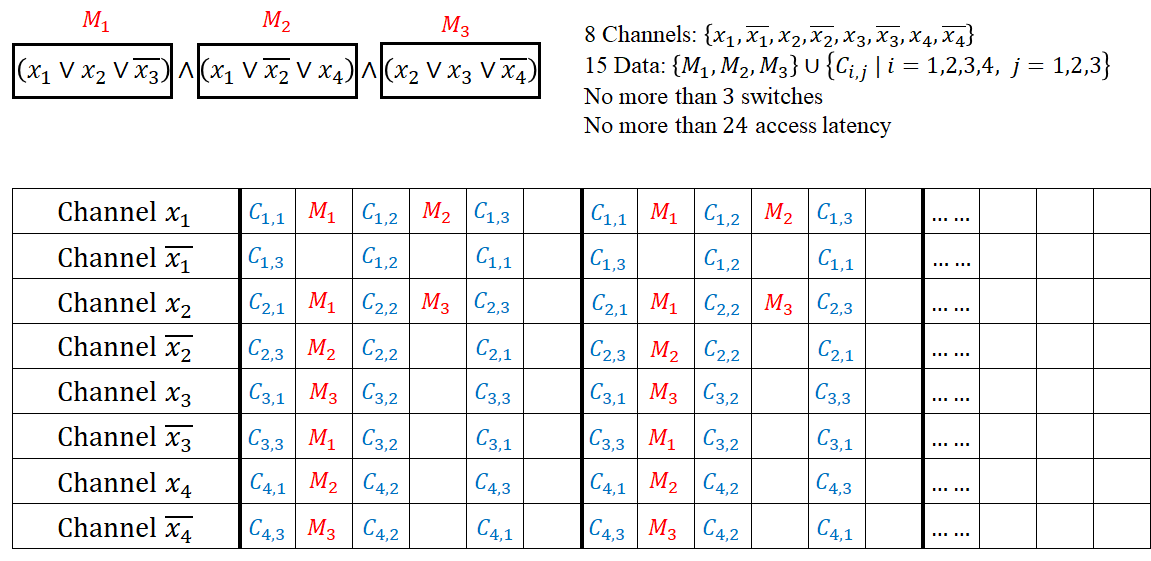
\includegraphics[width=7in]{MCDR-instance.png}\\
      \caption{The corresponding MCDR instance $\Sigma$}\label{fig: MCDR-instance}
    \end{figure}
    
    \textbf{Claim and Proof.} $\Sigma$ is satisfiable if and only if $\Phi$ is satisfiable. Here is the specific proof.
    \begin{itemize}
    \item \textbf{($\Longleftarrow$)} If $\Phi$ is satisfiable, then suppose the satisfying assignment of $\Phi$ is $y_1, y_2, \cdots, y_n$, where $y_i = x_i$ or $y_i = \overline{x_i}$ for all $i$. We can start at channel $y_1$, and move to channel $y_2$ at the end of the cycle in channel $y_1$, and then move to channel $y_3$ at the end of the cycle in channel $y_2$. Repeat this process $(n-1)$ times, so we can collect all the data items since $y_1, y_2, \cdots, y_n$ is the satisfying assignment of $\Phi$. We need to switch $(n-1)$ times, and actually we collect all the data items at the end of time $2n(L+1) - 1$. Both of them is within the constraints of switch number $h$ and access time $t$. Therefore, this is a satisfying solution to $\Sigma$. Hence, $\Sigma$ is satisfiable if and only if $\Phi$ is satisfiable.
    \item \textbf{($\Longrightarrow$)} If $\Sigma$ is satisfiable, then we can find a schedule which collects all the target data within the constraints of switch number $h$ and access time $t$. According to our design, \underline{we have to switch $(n-1)$ times to collect all the element data} because each element data is only in two channel. Moreover, we \underline{cannot access both channel $x_i$ and} \underline{channel $\overline{x_i}$} because it will cost one switch and we have no switch opportunity left. The access latency also restricts us to collect all the clause data in $n$ cycles. Suppose we visit channel $y_1$, channel $y_2$, $\cdots$, channel $y_n$, where $y_i = x_i$ or $y_i = \overline{x_i}$ for all $i$, then $y_1, y_2, \cdots, y_n$ should be a satisfying assignment of $\Phi$ since we have covered all the clauses. Hence, $\Phi$ is satisfiable if $\Sigma$ is satisfiable.
    \end{itemize}
    
    {\color{purple}\textbf{Note.} The original method of designing ascending order and descending order of the element data is to prevent switching in the middle of the cycle. In fact, we even do not need to constraint of switch number $h$ using this design (you can figure out the reason yourself). We \underline{do not use this property in our proof} because we have the constraint of switch number $h$, but \underline{it is a quite tricky design so I want to keep the design in the final solution}.}
    \end{proof}
    
    \begin{theorem}\label{MCDR-NPC}
    \emph{MCDR} problem is an NP-complete problem.
    \end{theorem} 
    \begin{proof}
    According to Theorem \ref{MCDR-NP}, we know that MCDR problem is an NP problem. Then according to Lemma \ref{3-SAT-REDUCE-MCDR}, we know that 3-SAT can be reduced to MCDR problem. Since 3-SAT is an NP-complete problem, MCDR problem should be an NP-complete problem.
    \end{proof}
    
\end{enumerate}

\textbf{Remark:} Please include your .pdf, .tex files for uploading with standard file names.




%========================================================================
\end{document}
